\chapter{FDI}
\label{chap:FDI}

\section{FDI trends}

Intro about studies of FDI in political science

Write about the economic literature on determinants of FDI

The political economy literature on the political determinants of FDI (and that
paper who shows that the political factors are not that important)

The studies on the preference of countries about FDI (Pandya, Pinto, and the
Harvard pub pol paper)


\section{Introduction}
\label{sec:introduction}

The political science literature on Foreign Direct Investment (FDI) has focused largely on how politics shapes the flow of FDI across countries. The central insight of this literature is that multinational corporations (MNCs) face an ``obsolescing bargain'' against the host government. Once the MNC has sunk its investment, it is vulnerable to the host government's changing regulations, backtracking on deals, or even expropriating its properties \citep{Li2009a, Sawant2010}. Certain institutional and political characteristics, such as numerous veto players, executive constraint, or strong property rights, allow the host government to make a credible commitment and thus ameliorate the severity of the ``obsolescing bargain'' problem \citep{Busse2007, Jensen2014, Li2003}. According to the literature, MNCs should invest more in countries with these characteristics.

This dominant approach in the literature has three long-standing issues that my paper will address. First, the majority of the literature relies on FDI stock and flow data as the outcome of interest even though they are often not an appropriate measure for the scale of MNCs' activities \citep{Kerner2014}. While it would be ideal to use firm-level data instead, both the lack of cross-national firm-level data and a suitable statistical model have posed a challenge.

Second, while there has been much focus on MNCs choosing host countries, the literature has largely neglected the other side of the investment decision: what are countries' preferences regarding MNCs? Consider the established finding that democracies receive more FDI. Without controlling for countries' preferences, it is difficult to interpret this fact as democracies actively pursuing MNCs or as MNCs finding democracies attractive. Not only are countries' preferences central to the modeling of investment decision, arguably it is also more steeped with politics and deserves more attention. \citet{Pinto2013} and \citet{Pandya2016} are two pioneering works in this area of research, proposing partisan politics and regime types as factors shaping countries' preferences for FDI. However, while their theories are ground-breaking, the empirical estimation of countries' preferences remains difficult.

Third, in addition to empirical issues raised above, I propose that we need to theorize about countries' preferences for FDI quality. While the political science literature has largely focused on the quantity of FDI, national policies and discourses pay much attention to the quality of FDI, using various incentives and restrictions to target certain types of FDI. Indeed, MNCs come with varying capital, demand for labor, and technology, all of which have different effects on the host country's economy. For example, policy makers and scholars have highlighted high-tech MNCs as a source of technological transfer for developing host countries, allowing them to upgrade their technical capacity and improve their productivity \citep{Findlay1978, Nunnenkamp2004}. While such high-quality FDI has been enthusiastically endorsed by the development community, I argue that only governments with a long time horizon want to attract high-tech FDI because technological transfer takes time to pay off.

In sum, the current literature would benefit from an analysis that is capable of using firm-level data to estimate both firms' and countries' preferences for each other's characteristics. To accomplish this goal, I adapt the two-sided matching model originally designed for the labor market and the marriage market. In this model, both firms and countries evaluate their available options and choose the best according to their utility functions. As in many social science contexts, we only observe the final firm-country matches and not the full set of available options (also known as the opportunity set). I solve this problem by using the Metropolis Hastings algorithm, a Markov chain Monte Carlo (MCMC) approach that repeatedly samples new opportunity sets and rejects them at an appropriate rate to approximate their true distribution. Since the two-sided matching model is derived explicitly from actors' utility functions, their parameters also enjoy a straightforward interpretation in the utility space instead of some aggregate outcomes.

The paper proceeds as follows. Section \ref{sec:literature_issues} discusses the
three long-standing issues with the literature and how they can be improved.
Section \ref{sec:model} lays out the utility structure in the two-sided matching
model and describes the matching process. Section \ref{sec:application} shows an
application of the model on a census of Japanese firms overseas. Section
presents the result. Section \ref{sec:conclusion} concludes.

\section{Three Issues in the Literature of FDI's Political Determinants}
\label{sec:literature_issues}

\subsection{Measuring MNCs' Activities}

For the majority of political science theory regarding FDI, the quantity of interest is the scale of MNCs' activities in a country, and not necessarily how much FDI crosses its border. Indeed, we theorize about how MNCs may reduce their activities for fear of expropriation, and how the host country's political factors can induce MNCs to invest more with a credible commitment not to expropriate. It is also the scale of MNCs' activities that determines how many jobs are created or how much of the domestic market is competed away, engendering labor's support and local business' lament.

However, to measure the scale of MNCs' activities, the vast majority of works uses how much FDI crosses the border, specifically FDI stock and flow \citep{Jensen2003, Ahlquist2006, Beazer2011, Graham2010}. As \citet{Kerner2014} points out, these measures, whose original purpose is to monitor balance of payments, are often misleading about MNCs' activities. FDI flow does not count locally raised capital and reinvested earnings since they do not cross any border. FDI stock calculated at market value fluctuates based on market price, unrelated to firms' behavior. FDI stock calculated at historical value, which records asset value at the time it was acquired, is more stable and appropriate to measure the scale of MNCs' activities. Unfortunately, due to onerous data requirements, most countries measures FDI stock by simply adding up FDI flow across years.

Given the interest of political science theory in MNCs' activities, \citet{Kerner2014} suggests less use of FDI stock and flow and more use of firm-level statistics. For example, consider the hypothesis that countries with more veto players have more stable policies and are thus more attractive to FDI \citep{Li2009a}. Instead of using FDI stock and flow into a country to measure its attractiveness, we can study whether more MNCs are located there.

While firm-level data has become more abundant in recent years,\footnote{Examples of firm-level data include the US Bureau of Economic Analysis (BEA)'s survey of all US firms abroad, Tokyo Keizai's Overseas Japanese companies database (\textit{Kaigai Sinshutsu Kigyou Souran}), World Bank's Enterprise Survey, and Orbis database of companies worldwide.} it is not clear how to analyze this type of data appropriately. Given the data structure of a set of firms interacting with a set of countries, one may consider a dyadic-based analysis, frequently used in the International Relations literature. In such analysis, the unit of observation is a firm-country dyad, and the model used is typically OLS regression. Each dyad is assumed to be independent of each other, and any bias caused by interdependency is fixed via post-estimation procedures, such as clustered standard errors \citep{Dorff2013}. 

Unfortunately, this dyadic approach is inappropriate to analyze MNCs' investment location. Once a firm chooses to invest in a country, it is by definition not investing in another. Therefore, the values of firm-country dyads deterministically constrain one another and cannot be modeled as independent draws from a common distribution.

The two sided matching model solves this problem by considering one firm-country match as the unit of observation. The intuition is as follows. If we observe that a firm is welcome to invest in countries $j_1, j_2, \dots, j_n$ but ends up investing in country $j^*$, it must mean country $j^*$ offers the highest utility to firms. Continuing the previous example, if country $j^*$ has more veto players than average, we can infer that MNCs indeed prefer countries with more veto players.

\subsection{Estimating Countries' Demand for FDI}

Recognizing that our model of investment location has not taken into account countries' demand for FDI, \citet{Pinto2013} and \citet{Pandya2016} recently broke ground in this area. Similar to the rich IPE literature in trade and exchange rate, these studies argue that countries' demand for FDI varies according to FDI's distributive effect on their domestic constituencies \citep{Broz2001, Milner2005a}. In this theoretical framework, labor supports FDI because foreign firms bring capital that increases the demand for labor and raises productivity, both of which lead to higher wage. On the other hand, domestic firms oppose FDI because foreign firms compete for local labor, inputs, and markets. Both \citet{Pinto2013} and \citet{Pandya2016} formulate their theories as a variant of this labor-vs-business tension, which surfaces in the former work as left-vs-right governments, and in the latter as democratic-vs-authoritarian regimes.

While these pioneering works have enriched our understanding of the relationship between politics and FDI, their empirical approaches do not satisfactorily measure countries' demand for FDI, leaving their theoretical arguments untested.

Consider \citet{Pinto2013}'s approach, which controls for economic and institutional factors that affect FDI flow into a country. The author then claims that the country's openness towards FDI is what's left in the residual.\footnote{Specifically, the estimation of FDI openness involves two steps. First, the author runs a gravity model explaining bilateral FDI flows, estimating the intercept as the host country-year fixed effect. Second, this fixed effect is then regressed on several economic and endowment factors of that country-year (i.e. GDP, GDP per capita, average school years, arable land). The residual in the second stage is considered the country's ``FDI openness'' in that year.} For this approach to be valid, every economic, institutional, and endowment factors that affect FDI flow have to be controlled for, leaving only the country's demand in the error term. This claim is much stronger than the regular assumption of exogenous and normally distributed error, which is valid as long as the omitted factors are uncorrelated with the independent variable of interest. Framed substantively, since the residual is likely to contain more than just the country's demand for FDI, if we observe an abnormally high level of FDI, we do not know whether it is because the country welcomes FDI or because MNCs find something attractive in the country.\footnote{In addition, the data requirement of bilateral FDI flows, ideally disaggregated by sectors, is very demanding. Therefore, this approach is limited to OECD countries only \citep{Pinto2008}. During the period the authors study, 1980-2000, OECD countries accounted for 95\% of global FDI outflow and 90\% of inflow. However, since then the role of the developed world in global FDI has declined sharply, reduced to 60.8\% of outflow and 40.6\% of inflow in 2014 \citep{UNCTAD2015}.}

In contrast to \citet{Pinto2013}'s statistical approach, \citet{Pandya2014, Pandya2016} substantively measures countries' demand for FDI, using the annual US Investment Climate Reports to code the number of industries that have foreign ownership restrictions or face investment screening. The advantages of this measurement are its ease of interpretation and its availability for many countries. However, two problems remain. First, adding up the raw count of restricted industries is not appropriate because industries are not all the same. For example, given the reach of the banking sector into all corners of the economy, a country's opening up its financial industry indicates much more FDI-friendliness than, say, allowing foreign furniture makers to set up shops. Since the theoretical argument is driven by FDI's distributive effect, it is suspect to ignore the varying impact of FDI across sectoral constituencies. 

Second, according to the coding rules, an industry is coded as free if there is
no mention of restriction. If an industry receives little FDI, it may not be
worth mentioning as being restrictive and yet still coded as open. Therefore,
``zero restriction'' in the dataset can either mean that a country is very
closed or very open to FDI. This concern is not hypothetical. Figure \ref{fig:china_fdi_restriction} shows that, following the coding of the US Investment Climate Reports, China seemed 100\% open to FDI up until 1986 when it started imposing restrictions. The reality is the opposite. Prior to 1986, only limited FDI was allowed as joint-venture in Special Economic Zones (SEZ). The year of 1986 was, in fact, the first time China allowed any wholly owned FDI outside of SEZs.

\begin{figure}[!ht]
\centering
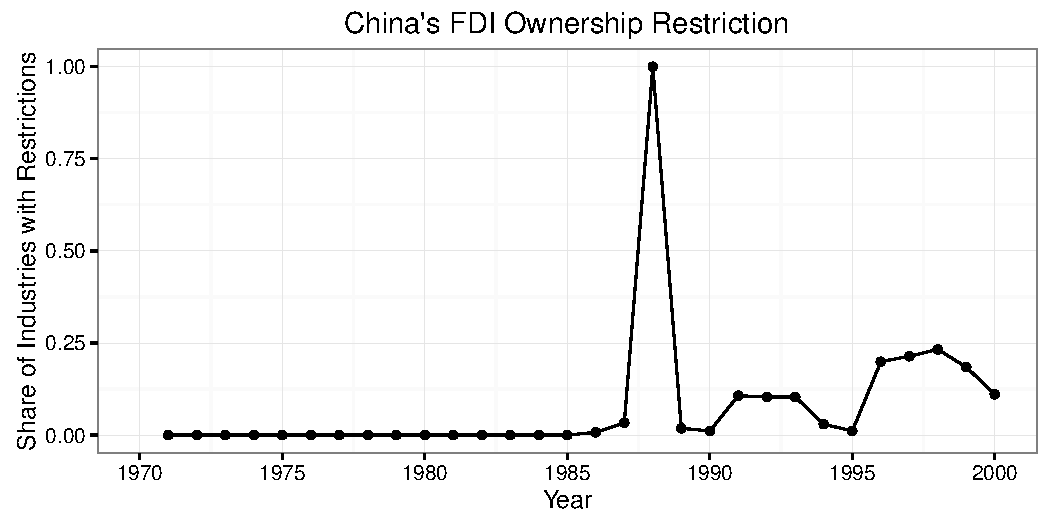
\includegraphics[width=0.75\textwidth,keepaspectratio]{../figure/china_fdi_restriction}
\caption{China's FDI Ownership Restriction, as coded in \citet{Pandya2010}. Prior to 1986, FDI in China was limited to few experimental Special Economic Zones, and thus not mentioned in US Investment Reports. The sharp spike in 1988 also does not seem to correspond to any actual change in policy, and likely another artifact of reporting. (See \citet{Zebregs2002} for a historical overview of China's FDI policy.)}
\label{fig:china_fdi_restriction}
\end{figure}

The two-sided matching model circumvents these thorny measurement issues by incorporating countries' utility function directly into the model. If we observe that country $j$ welcomes firms $i_1, i_2, \dots, i_n$ to invest but not others, we can compare the characteristics of firms $i_1, i_2, \dots i_n$ with the others to infer country $j$'s preference.


\subsection{Estimating Countries' Preferences for FDI's Technological Intensity}

While the political science literature has focused almost exclusively on the quantity of FDI, treating all FDI as one homogeneous flow of capital, policy makers seem to pay much more attention to distinguishing types of FDI. Commenting on the role of International Investment Agreements (IIAs), \citet{UNCTAD2015} says, ``Today, increasing the quantity of investment is not enough. What matters is its quality, i.e. the extent to which investment delivers concrete sustainable development benefits.'' Governments in developing countries, from Ghana to China, all offer various forms of tax incentives and fee waivers to attract FDI that invests in a remote region, brings new technology, or focuses on exporting \citep{Ricupero2000}. Since 2006, China's official FDI policy has been ``quality over quantity,'' promoting FDI with intense R\&D in high-productivity sectors \citep{Guangzhou2011}. Indeed, for developing countries, the hope is that MNCs will transfer their technologies to the domestic economy by training workers or partnering with local suppliers.

Despite the importance of disaggregating FDI by its quality, data unavailability remains the bottleneck. The few existing attempts use detailed data from only one country or limit the sample to OECD countries \citep{Alfaro2003, Alfaro2007, Javorcik2004}. With cross-country firm level data now available, we often have information on the firms' industry or even research and development (R\&D) expenditure. With the two-sided matching model, I will be able to estimate countries' preferences for firms' technological intensity. I hypothesize that, since MNCs' technologies takes time to diffuse to local businesses, a country' preference of high-tech FDI is shaped by its time horizon.

\section{Using firm level data in FDI studies in Political Science}

Look at Kerner2014

Look at studies in FDI across China

\section{The literature on Japanese MNCs investment}

Make a graph about the size of Japanese FDI relative to Asia FDI here

Calculate the size of Japanese FDI into several countries (nominator from JETRO,
denominator from IMF)

Relative exchange rate (Takagi2011). Assume that the capital market is
imperfect, that external borrowers face a premium. So if a host country currency
depreciates, inflow FDI will increase because the same amount of source currency
can buy more input in the host country. The relationship is especially strong
between exchange rate and inflow of FDI into industries with a lot of
firm-specific assets. (e.g. Japanese firms buy a US firm with innovation for
cheap, then use that innovation to improve its production back home in yen) 

(Originally people don't think exchange rate matter because if you can buy an
asset for cheap in the host country, when you repatriate the profit back to the
home country it's a wash)

FDI is all about the relative factors (because a firm thinks about a country in
terms of how that country is relative to its host). So the two sided matching
framework makes sense

General FDI: Why don't firms export or license, but open their own plant
overseas? Argument is that they have firm-specific asset that cannot be fully
exploited otherwise. A licensee won't be able to exploit the entire asset, both
sides can't agree on a price beforehand (This is the OLI framework,
ownership-location-internalization, also the internationalization hypothesis). Empirically, firm specific asset is
unobservable, so people use R\&D intensity and advertising intensity instead.
R\&D does correlate strongly with multinationality.


\section{Applying the Two-Sided Matching Model to Japanese MNCs}
\label{sec:application}

In this section, I apply the two-sided matching model to study the investment
location of Japanese firms overseas. The data comes from a dataset compiled by
Andrew Delios from \textit{Kaigai
  Shinshutsu Kigyou Souran} (Japanese Overseas Investments-by Country), between
1986-1999 editions, a publication that contains information
about the foreign affiliates of listed Japanese firms.\footnote{I thank Professor Andrew Delios for
  generously sharing the data.} Tokyo Keizai, Inc. collect these data via annual
surveys of the overseas operations of both listed and non-listed firms. This database is reputed to include all Japanese
firms overseas \citep{Yamawaki1991}. \citep{Delios2001} compares the coverage of
the Japanese Overseas Investment with other sources of publicly listed firms and
found that 98.5\% of public firms are included, which has 99.5\% of the foreign
subsidiaries. Since there is no public information on non-public firms, they
cannot check the coverage of the Japanese Overseas Investment for these firms.
However, the result for the public firms makes us confident that our data is
close to the population of Japanese FDI overseas.\footnote{There are similar
  datasets if scholars want to replicate this study in other context. On a
  global scale, the ORBIS dataset claims to have data of FDI firms across
  countries. (cite the paper that I reviewed). However, there are concerns about
  its data quality, given that the data is collected via public governmental or
  municipal sources. Due to the differences of reporting across jurisdiction,
  the data quality is much less consistent than the Japanese Overseas Survey. For the US, there is a census of
  US firms overseas, which should be similarly high quality. However, this
  dataset requires citizenship. Tokyo Keizai, Inc. also continue to publish this
data series. However, the cost is prohibitive and require understanding Japanese
to work with.}



Sample choices:

- I only use the data of subsidiaries that are founded in year 1996 (which is
different from the list of companies who are in existence in year 1996). Reasons:
+ the utility function is only modeled as a linear combinations of the country /
firms covariates. It does not take into account the cost of uprooting a firm to
move to another country once they are already there. This is important for FDI
because, unlike equity investor, FDI are less foot-loose. Indeed, the fact that
it is not footloose is an important quality of FDI that's appealing to countries
(cite). The political economy literature on FDI has also derived its insights
largely from this ``obsolescing bargain'' problem, so it's important that our
model takes this into account. In past applications of the two sided matching
approach, researchers use a random sample in time (i.e. a sample of all couples
who's married in a certain year), which is fine, because the
cost of leaving a job or leaving a partner may not be too onerous. However, for
FDI, this fixed cost is more central. By limiting the sample to the firms who
are founded in 1996, we examine their decisions as they are all looking for
potential locations.\footnote{Of course, a subsidiary's foundation year in 1996
  does not preclude the decision process to happen outside of this year.
  However, I consider this a reasonable approximation, given that many country
  characteristics, especially the political and institutional ones, do not
  change drastically within a window of several years.}

+ the data is largest for this year. (some summary statistics here). There may
be some concerns about this year being a special year, in the year leading up to
the 1997 Asian Financial Crisis. But 1) we're only looking at manufacturing
firms, not equity investors or land developers, 2) FDI during the crisis is
largely the same as before the crisis \citep{UNCTAD1998}. Indeed, this is
because FDI firms are largely looking at countries' fundamentals, such as labor
cost, market potential, and thus not affected by the fluctuations in the
financial markets. Essentially, the types of firms that invest before, during,
and after crisis are still the same types of firms.\footnote{One potential
  concern is that our data does not capture the firms who thought about making
  an investment but decided not to. This could be a problem if the MNCs in our
  dataset is the most risk-seeking firms, then essentially we've only estimated
  the preference of the very risk-seeking or the very risk-averse firms. AFC too
high short term interest, too high local currency that is fixed. However, the
exit rate of Japanese firms in Thailand, the epicenter of the financial crisis,
is the same, indicating that the types of firms who invest are not so affected
by the financial crisis. Looking at the exit is the reverse way of looking at
who would have invested but didn't. \citep{Delios2001}}

+ I only consider Japanese FDI into East Asian and Southeast Asian economies to
make sure that it's realistic to say that all these companies have the same
preference parameters. \citep{Pak2005} finds that Japanese FDI in the West seeks
to augment their global competitiveness, while Japanese FDI in the East focuses
on exploiting their core competencies. Japanese FDI in the West are ones with
oligopolistic power in their domestic market (so they are in a strong position
to compete) and require R\&D and marketing capabilities. They have different
level of equities. This suggests that the two types of firms are fundamentally
different.\footnote{Even though the difference in theory could be due to the
  preference of the countries. However, it doesn't make sense why the level of
  Japanese ownership is also different (because countries would not care about
  this).} 

The final sample includes 6474 Japanese
foreign affiliates in 2003, spreading across 37 countries, with China and the US
leading as the two top destinations for Japanese MNCs (Table \ref{tab:list_of_countries}).

For firms' characteristics that countries consider, I include:

\begin{itemize}
\item Capital size (in US\$): A main argument for the benefit of FDI is that it brings capital to the country, improving labor productivity. MNCs' capital is especially important for developing countries, which cannot muster much domestic capital from their poor population. The capital size of a firm is included in the Japanese Overseas Business dataset.

\item Labor size: Similarly, a reputed benefit of FDI is that it creates jobs, generating not just economic growth but also increasing the government's popularity among the populace. The total number of employees of a firm is included in the Japanese Overseas Business dataset.

\item Technology intensity: I proxy for a firm's technology intensity by the
  industry to which it belongs. \citet{OECD2009} categorizes ISIC industries
  into four levels of technology intensity---low, medium low, medium high, and
  high---according to the level of R\&D expenditure divided by sales. I convert
  the industry classification of firms in my data from SIC 3 to ISIC and
  categorize their technology intensity from 1 to 4, with 1 being low and 4
  being high. On several occasions, one industry in SIC 3 matches to multiple
  ISIC (rev 3) industries or none at all. In the former case, I take the average
  across matched ISIC industries. In the latter case, the data is missing and
  later removed from the analysis.\footnote{\cite{Bergstrand2007} discusses the
    difference between R\&D intensity and advertising intensity, and find that
    R\&D intensity is higher for manufacturing firms compared with consumer
    product firms. Plus R\&D intensity is much more important for firms'
    performance than advertising intensity.}\footnote{Definition of R\&D
    intensity: the amount spent on R\&D as a percentage of sale}

\item Export intensity (ratio of export to sale):
\end{itemize}

Summary statistics table for these covariates.


For countries' characteristics that firms consider, I include:

\begin{itemize}
\item Market size: MNCs are expected to prefer countries with a large market
  size, which present MNCs with many potential customers. Indeed, this has been
  often cited as the allure of China to MNCs \citep{Luo2010}, as well as
  confirmed in larger studies. This is also a major variable in the gravity
  model, which has become a standard model for analyzing FDI flows.
  \citet{Bergstrand2007} provides the theoretical framework for the use of
  gravity model. I follow the standards in the literature and include log GDP
  (constant 2005 US\$), taken from the Penn World Table.\footnote{An advantage
    of the Penn World Table is that it compiles data for Taiwan, an important
    destination that the World Bank Development Indicators does not include.}

\item Level of development: MNCs are expected to prefer countries with a high
  level of development. A developed economy has consumers with high purchasing
  power and better infrastructure. It can also measure capital abundance, in
  which case a higher GDP per capita imply less flow because the simple model of
  FDI frames FDI as the movement of capital from the capital rich countries to
  the capital poor countries. To measure development, I use log GDP per capita
  (constant 2005 US\$) from World Development Indicators.

\item GDP growth may be a proxy of potential returns, 

\item Labor quality: As one primary factor of production, labor matters greatly to firms' productivity and profit. To measure labor quality, I use the average years of schooling of adult, taken from the UNDP's Human Development Report.\footnote{Since Taiwan is not included in UNDP's and World Bank's data, I collected its statistics from the Taiwanese Statistical Website.}

\item Democracy: Democracy has been a mainstay in the political science literature on FDI. Scholars have argued that MNCs want to invest in democratic regimes for various reasons, including stable policy, credible commitment, and strong property rights \citep{Ahlquist2006, Li2003, Jensen2003}. On the other hand, recent works have also argued that democratic regimes want FDI more than autocratic regimes \citep{Pandya2016}. Thus, it is unclear whether the observed high level of FDI in democracies is due to the push or the pull factors. By controlling for countries' preference in the two-sided matching model, I can better estimate the effect of democracies on firms' utility. I measure democracy using the binary Demoracy \& Dictatorship, developed by \citet{Cheibub2009b}.
\end{itemize}


\section{Conclusion}
\label{sec:conclusion}

In this paper, I propose the two-sided matching model to estimate firms' and countries' preferences, solving three persistent issues in the literature of FDI's political determinants. The results indicate that, for Japanese MNCs, only a country's level of development matters and not its market size, labor quality, or regime type. This finding suggests that we should take a closer look at the relationship between democracies and MNCs. Since previous works in the literature have not controlled for countries' preferences, they may have mistaken democracies' love for FDI as FDI's fondness for democracies.

On the other hand, the model's estimation of countries' preference remains lacking. Since each country has its own set of parameters, the parameter space seems too large for the current implementation of the Metropolis-Hastings algorithm to fully explore. Several solutions are possible. First, we can collapse countries into categories of interest, e.g. regime types, (categorical) time horizon length. Second, we can build a hierarchical model, modeling countries' preferences as draws from a common distribution. Such model will allow us to pool information across countries and reduce the parameter space.